\chapter{Introducción}\label{cap.introduccion}
En este capítulo se definirá el contexto en el cual se sitúa este proyecto así como la motivación principal que ha llevado a desarrollarlo. Se explicará de forma general qué es la robótica, sus aplicaciones y algunos softwares utilizados para la programación de robots. También se expondrá su uso en docencia hoy en día y se comentará de manera general la plataforma JdeRobot-Academy.

\section{Robótica}
La robótica es una rama de la ingeniería que emplea la informática para diseñar y desarrollar sistemas que permitan facilitar la vida del ser humano, e incluso sustituirle en determinadas tareas. Esta rama usa conceptos de diversas disciplinas, tales como la física, las matemáticas, la electrónica, la mecánica, la inteligencia artificial o la ingeniería de control. Mediante todas estas disciplinas realiza diversas máquinas que ejecutan diferentes comportamientos en función de su propósito. Estas máquinas se denominan ``robots''. En el futuro, dominar esta disciplina será clave debido a que cada vez de forma más habitual se implantan robots en diferentes empleos, como pueden ser las cadenas de automatización. \\

\subsection{Historia de la robótica}
El término ``robot'', viene de la palabra checa ``robota'', cuyo significado es ``trabajo forzado''. Dicha palabra fue introducida por primera vez por el dramaturgo y autor checoslovaco Karel Capek (1890 – 1938), en su obra de teatro R.U.R (Robots Universales de Rossum) en 1921. Con este libro surgió la palabra ``robótica'', pero entonces era un término de ciencia ficción. En base a este término se puede decir que un robot es una máquina programada para moverse, manipular objetos y realizar trabajos, para lo cual debe interaccionar con el entorno que le rodea.\\

Unos años más tarde Isaac Asimov (1920 – 1992) introdujo conceptos acerca de la robótica. Isaac Asimov era un escritor y bioquímico estadounidense nacido en Rusia, el cual publicó el libro ``Yo Robot'' en 1950. Este libro contenía tres leyes de la robótica:

\begin{enumerate}[1.]
    \item Un robot no puede lastimar a un ser humano o permanecer inactivo ante un daño que se le pueda hacer.
    \item El robot debe obedecer al ser humano excepto si contradice la primera ley.
    \item El robot debe proteger su existencia salvo que entre en conflicto con las leyes anteriores.
\end{enumerate}

Con este libro, Isaac Asimov consiguió que la robótica se hiciera popular. Sin embargo, no fue hasta mediados de siglo cuando los robots empezaron a disponer de un sistema de control propio. Hasta entonces eran controlados por seres humanos. \\

En los años 50, los primeros robots móviles fueron construidos por Grey Walter (1910 – 1977). Estos robots eran conocidos como tortugas de Bristol y empleaban válvulas, sensores de luz y detectores de contacto, capaces de evitar obstáculos. También, George Devol (1912 – 2011) patentó el primer robot programable y creó la primera empresa dedicada a la robótica llamada Unimation (Universal Automation) junto con Josef Engelberger (1925 - 2015). \\

En la década de los 70, se desarrolló el robot JPL Rover en la Jet Propulsion Laboratory en Pasadena. Su principal fin era la exploración espacial empleando una cámara de televisión, un láser de telemetría y sensores táctiles. Además, Hans Moravec (1948) diseñó CART en Stanford. Este robot evitaba obstáculos mediante una cámara. Para ello creaba un modelo bidimensional de su alrededor a partir de nueve fotos tomadas del entorno. \\

En los años 80, en la Universidad de Stanford, surgen robots capaces de procesar dos cámaras estéreo. Estos robots son capaces de realizar una reconstrucción 3D. 
En el año 2000, Honda lanza el robot Asimo. Este humanoide pretende ayudar a las personas que carecen de movilidad completa, así como animar a la juventud para estudiar ciencias y matemáticas.\\

\begin{figure}[H]
  \begin{center}
    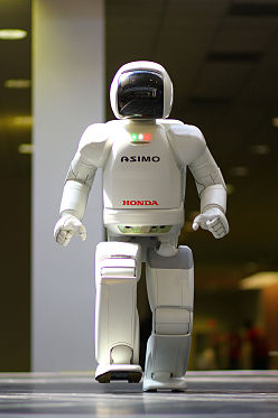
\includegraphics[width=0.2\textwidth]{figures/Introduccion/asimo.png}
		\caption{Robot Asimo}
		\label{fig.asimo}
		\end{center}
\end{figure}

\subsection{Aplicaciones de la robótica}
Actualmente la robótica está en continua expansión. Se pueden encontrar robots en diferentes áreas y entornos. Una de las principales áreas donde se encuentran robots es en la industria. Gracias a los robots se pueden elaborar tareas peligrosas y complejas. El robot industrial, debido a su naturaleza multifuncional puede llevar a cabo un gran número de tareas, totalmente inalcanzable si la mano de obra es humana de manera que se abarata mucho el coste de producción. \\

En el mundo del automóvil se han introducido robots tanto para su construcción, utilizando brazos mecánicos en las cadenas de montaje, como para lograr que los coches sean autónomos. Una de las empresas pioneras en este ámbito es Google que junto con Fiat-Chrysler han desarrollado el proyecto ``Waymo''. Estos vehículos autónomos tienen sensores y software diseñado para detectar personas, ciclistas, vehículos, ciclistas y carreteras a una distancia mayor que dos campos de fútbol en todas las direcciones. \\

\begin{figure}[H]
  \begin{center}
    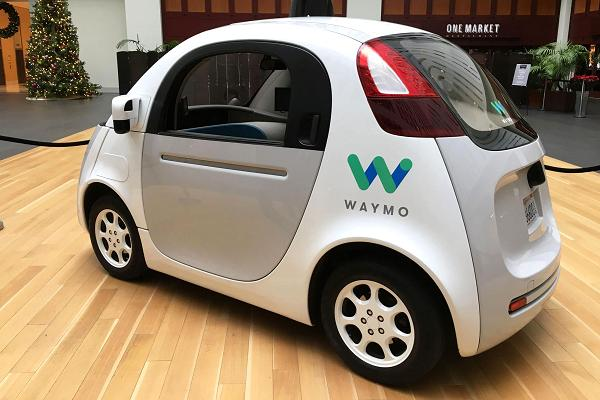
\includegraphics[width=0.4\textwidth]{figures/Introduccion/waymo.jpg}
		\caption{Coche autónomo Waymo}
		\label{fig.waymo}
		\end{center}
\end{figure}

La empresa Tesla también ha desarrollado coches autónomos. Sus coches tienen instaladas ocho que ofrecen una visión de 360 grados alrededor del vehículo en un área de hasta 250 metros. Además, dispone de doce sensores ultrasónicos capaces de detectar objetos de todo tipo y tamaño alrededor del coche, y de un radar delantero que ofrece datos adicionales.

\begin{figure}[H]
  \begin{center}
    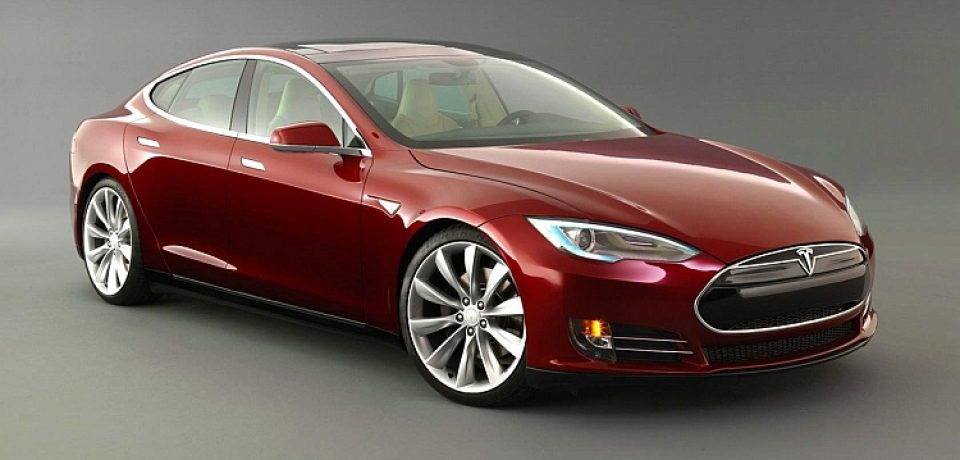
\includegraphics[width=0.4\textwidth]{figures/Introduccion/tesla.jpg}
		\caption{Coche autónomo Tesla (Model S)}
		\label{fig.tesla}
		\end{center}
\end{figure}

El objetivo de los coches autónomos es evitar los accidentes de tráfico y disminuir los atascos. \\

Hoy en día también se pueden encontrar robots en los hogares de las personas, como por ejemplo con aspiradoras autónomas. Estas aspiradoras mediante sensores y el desarrollo de tecnologías en ámbitos como el diseño de mapas y de sistemas de navegación son capaces de limpiar las casas de una manera fiable y robusta ante distintos tipos de obstáculos como muebles o escaleras. La empresa iRobot es pionera mundial en este sector de la robótica con su aspiradora Roomba, aunque también se pueden encontrar otras aspiradoras potentes en el mercado como el robot aspirador Dyson que calcula un patrón de sistema sistemático y de esa forma sabe por dónde ha pasado y dónde tiene que ir a limpiar.\\

\begin{figure}[H]
  \begin{center}
    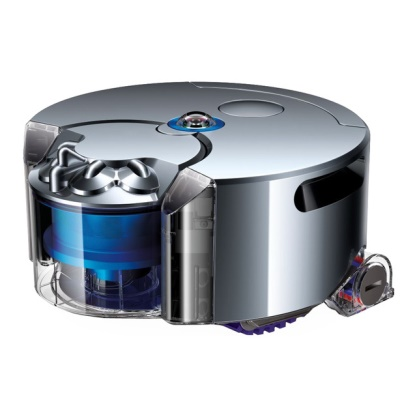
\includegraphics[width=0.3\textwidth]{figures/Introduccion/dyson.jpg}
		\caption{Robot aspirador Dyson}
		\label{fig.dyson}
		\end{center}
\end{figure}

Amazon, en sus almacenes, también ha introducido robots para que la logística sea mucho más rápida y eficaz. Utiliza la automatización para almacenar y retirar los productos. Sus robots son capaces de cargar hasta 1300 Kg y mediante el uso de un láser y una cámara en la parte delantera, son capaces de detectar obstáculos. Se mueven a 1,7 metros por segundo y realizan un pedido en 15 minutos en vez de en 70, disminuyendo así el tiempo de entrega de sus productos.

\begin{figure}[H]
  \begin{center}
    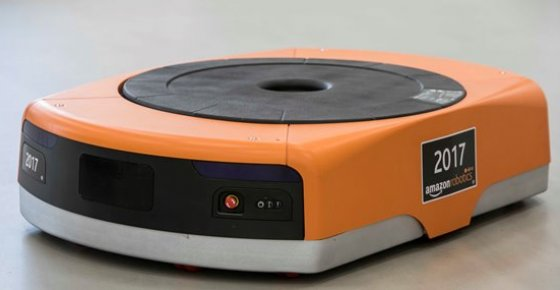
\includegraphics[width=0.3\textwidth]{figures/Introduccion/amazon.jpg}
		\caption{Robot de Amazon Drive}
		\label{fig.amazon}
		\end{center}
\end{figure}

También se pueden encontrar robots en otra gran variedad de ámbitos como en laboratorios de investigación, en la medicina, en el ejército, etc. 

\subsection{Clasificación de robots} 
En función al software desarrollado en el controlador, al diseño mecánico y a la capacidad de los sensores, los robots pueden clasificarse de acuerdo a su arquitectura, su aplicación, su nivel de inteligencia, su generación, su nivel de control y su nivel de lenguaje de programación.

\begin{itemize}
    \item Según su cronología:
    \begin{itemize}
         \item Primera generación: En este grupo se engloban sistemas mecánicos multifuncionales que poseen un sistema de control manual, de secuencia fija o de secuencia variable. Mediante instrucciones programadas de forma previa realizan tareas. Dichas tareas se efectúan secuencialmente. Los robots de primera generación no consideran las posibles modificaciones que se producen en su entorno. 
         \item Segunda generación: Estos robots son más conscientes de su entorno que los robots de primera generación. Dichos robots poseen sensores por medio de los cuales obtienen información acerca de su entorno. De esta forma son capaces de actuar y adaptarse en función a los datos analizados. Dos características muy importantes de estos robots son su capacidad de aprendizaje y de memoria. Pueden memorizar los distintos movimientos que desean realizar.
         \item Tercera generación: Los robots son capaces de llevar a cabo las órdenes de un programa. Para ello cuentan con controladores que utilizan la información que les proporcionan los sensores. A diferencia de los robots de primera generación, son muy conscientes de su entorno y esto les permite adaptarse.
         \item Cuarta generación: Los robots se pueden considerar “inteligentes”, ya que pueden aprender acerca del entorno que les rodea, y desenvolverse adecuadamente empleando distintos métodos de análisis y obtención de datos. Estas estrategias tan complejas de control son posibles debido a los sensores que son empleados, que son bastante más sofisticados que en otras generaciones. Debido a todas estas mejoras, los robots son capaces de supervisar su entorno y basarse en datos más sólidos. Además, en ciertas situaciones son capaces de actuar correctamente, ya que se basan en modelos.
    \end{itemize}
    \item Según su arquitectura física:
    \begin{itemize} 
    	\item Poliarticulados: Son robots estáticos, aunque en algunas ocasiones pueden realizar desplazamientos limitados, y mover sus extremidades en un espacio de trabajo concreto mediante algún sistema de coordenadas y con un limitado número de grados de libertad. Estos robots pueden ser muy diferentes en su forma y configuración. Se emplean habitualmente en zonas de trabajo amplias o alargadas. Los robots industriales, manipuladores y cartesianos son algunos ejemplos.
		\item Móviles: Son robots con una importante capacidad de desplazamiento. Son capaces de realizar un cierto desplazamiento, mediante la información que les proporcionan sus sensores del entorno o mediante tele-mando. Suelen tener un sistema locomotor de tipo rodante. Estos robots son capaces de evitar obstáculos y tienen un nivel de inteligencia considerablemente alto. Se suelen emplear para transportar piezas en una cadena de fabricación.
		\item Androides: Estos robots intentan imitar de manera parcial o total la forma y el comportamiento del movimiento humano. No son muy prácticos, y son poco evolucionados. Su principal uso es el estudio y la experimentación.
		\item Zoomórficos: La principal característica de estos robots es su sistema de locomoción, el cual pretende imitar a los distintos seres vivos. Existen dos categorías principales: caminadores y no caminadores.
		\item Híbridos: Los robots híbridos son difíciles de clasificar puesto que su estructura está formada por la combinación de alguna de las arquitecturas anteriores.
	\end{itemize}
	\item Según su aplicación:
	\begin{itemize}
		\item Robots médicos: La aplicación fundamental de estos robots se sitúa en el campo de la cirugía. Es fundamental que los diversos brazos robóticos que se emplean en alguna operación quirúrgica sean lo suficientemente precisos. Estos robots pueden ser controlados a distancia. 
		\item Robots industriales: Son robots automáticos, reprogramables y con múltiples funciones. Estos robots poseen tres o más ejes para poder orientar y colocar en la posición correcta diferentes piezas, materiales, dispositivos o herramientas. Son empleados en la realización de diferentes trabajos de la producción industrial en sus diversas etapas. La principal característica del ambiente de trabajo de dichos robots es el control del entorno, esto hace que las funciones de los robots se simplifiquen de manera notable. 
		\item Robots militares: Estos robots tienen aplicaciones militares concretas, para las cuales pueden actuar de forma autónoma o estar controlados de forma remota. Presentan diferentes morfologías en función de su uso. Dichos robots asisten o guían al ejército en operaciones especiales. Sus funciones pueden ser la búsqueda, el transporte, el rescate o el ataque.
		\item Robots educativos: Estos robots se crearon con el fin de emplearse de forma educativa, especialmente en escuelas e institutos. Los robots educativos de LEGO Mindstorms son especialmente usados en las escuelas.
		\item Robots de servicio: De forma habitual, este tipo de robots se emplean para reemplazar al ser humano en entornos no controlados, hostiles y donde puede ser necesario un cambio de forma del robot. Son dispositivos electromecánicos controlados por ordenador y normalmente dotados de movimiento. Suelen poseer uno o varios brazos mecánicos independientes. No realizan tareas industriales.
		\item Robots de investigación: Este conjunto de robots son empleados habitualmente en los laboratorios de las Universidades. Están destinados a la investigación y por ello pueden ser de muy diversas formas. Estos robots pueden tener un fin concreto en algún proyecto de investigación o no tener ninguna aplicación concreta.
	\end{itemize}
\end{itemize}


\section{Software para robots}
Mediante el software se le indica al robot las acciones que tiene que realizar, dotándole así de inteligencia y autonomía. Este desarrollo de software suele ser complicado y arduo. En la actualidad, se han propuesto muchos sistemas de software y frameworks o entornos, para hacer más fácil la programación de los robots. 

\subsection{Middleware}
Los robots autónomos son sistemas complejos que requieren de la interacción entre numerosos componentes heterogéneos como son el software y el hardware. Debido al aumento de la complejidad de las aplicaciones robóticas y la diversa gama de hardware, el middleware robótico está diseñado para gestionar la complejidad y la variedad del hardware y las aplicaciones. Permiten a una aplicación interactuar o comunicarse con otras aplicaciones, sistemas operativos, redes o hardware. Los middlewares robóticos proporcionan una API (Interfaz de Programación de Aplicaciones) que simplifica la comunicación entre las aplicaciones robóticas y la heterogeneidad del hardware del robot, como por ejemplo los sensores, simplificando así el diseño del software y mejorando su calidad. 

\begin{figure}[H]
  \begin{center}
    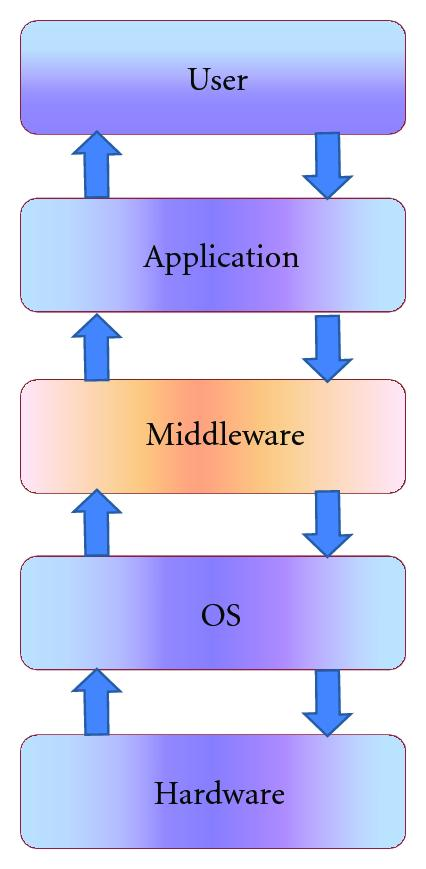
\includegraphics[width=0.3\textwidth]{figures/Introduccion/middleware.jpg}
		\caption{Estructura del funcionamiento del middleware}
		\label{fig.middleware}
		\end{center}
\end{figure}

Algunos de estos middlewares robóticos son:

\begin{itemize}
	\item \acrfull{ros} \footnote{\url{http://www.ros.org/}}: Es el software más usado en el mundo para la programación de robots. Es un entorno de programación de código abierto mantenido por la Open Source Robotics Foundation (OSRF). Ofrece una colección de herramientas, bibliotecas y convenciones que tienen como objetivo simplificar la tarea de crear un comportamiento robótico complejo y robusto en una amplia variedad de plataformas robóticas. La librería está orientada para un sistema UNIX (Ubuntu (Linux)), aunque también se está adaptando a otros sistemas operativos como Fedora, MacOS-X, Arch, Gentoo, OpenSUSE, Slackware, Debian o Microsoft Windows, considerados como ``experimentales''.
	
	\item Orca \footnote{\url{http://orca-robotics.sourceforge.net/}}: Es un entorno de programación usado para desarrollar sistemas robóticos basados en componentes. Utiliza una biblioteca de código abierto para la comunicación y la definición de interfaces. Todos sus componentes están escritos en C ++ y tiene ejemplos en Java, Python y PHP. Da soporte completo para Linux. Además, interfaces, bibliotecas principales y algunos componentes se compilan en Windows XP y hay compilaciones experimentales en MacOS-X.

	\item Player/Stage Project \footnote{\url{http://playerstage.sourceforge.net/}}: Es un proyecto que desarrolla software libre que permite la investigación de robots y sensores. Su servidor es uno de los interfaces de control de robots más utilizados del mundo, así como sus backends de simulación, Gazebo y Stage. Su modelo cliente-servidor permite que los programas de control del robot se escriban en cualquier lenguaje de programación y se ejecuten en cualquier ordenador con una conexión de red al robot. Es compatible con una amplia variedad de robots y accesorios móviles como el robot Kinect de Microsoft o la aspiradora Roomba de iRobot. Player Project funciona en Linux, Solaris, * BSD y Mac OSX (Darwin).

	\item RT-middleware \footnote{\url{http://www.openrtm.org}}: Tiene como objetivo establecer una plataforma basada en la tecnología de objetos distribuidos. RT-middleware soporta la construcción de varios sistemas robotizados en red mediante la integración de varios elementos robóticos habilitados para dicha red, denominados RT-Components. Los sistemas robóticos a los a los que da soporte no son necesariamente robots de un solo cuerpo, como robots móviles o robots humanoides, sino más generalmente ``cualquier sistema de red inteligente que utilice tecnología robótica y que pueda realizar tareas en el mundo real''. Por ejemplo, esto también incluye sistemas que aunque no se parecen a los robots utilizan tecnología robótica, como un soporte de vida diaria o sistemas de enfermería en los que varios sensores y actuadores colaboran a través de una tecnología de redes. Da soporte para Linux y Windows y tiene versiones en C++, Java y Python.

	\item JdeRobot \footnote{\url{http://jderobot.org}}: Es un entorno de programación utilizado para desarrollar aplicaciones en robótica y visión por computadora. Ha sido diseñado para ayudar en la programación de software inteligente. Principalmente, está escrito en C++ y proporciona un entorno de programación basado en componentes distribuido en el que el programa de aplicación está compuesto por una colección de varios componentes asincrónicos concurrentes. Los componentes pueden ejecutarse en diferentes equipos y están conectados mediante el middleware de comunicaciones ICE (Internet Communications Engine). Los componentes pueden escribirse en C++, Python o Java y todos ellos interactúan a través de interfaces ICE.

\end{itemize}

\subsection{Bibliotecas}
En informática, una biblioteca es un conjunto de implementaciones funcionales, codificadas en un lenguaje de programación, que ofrece una interfaz bien definida para la funcionalidad que se invoca. Su fin es ser utilizada por otros programas, independientes y de forma simultánea. Las bibliotecas pueden vincularse a un programa (o a otra biblioteca) en distintos puntos del desarrollo o la ejecución de dicho programa. Algunas de las bibliotecas utilizadas en robótica son:

\begin{itemize}
	\item OpenCV \footnote{\url{http://opencv.org/}}: Es una biblioteca libre de visión artificial originalmente desarrollada por Intel. Contiene más de quinientas funciones que abarcan una gran gama de áreas en el proceso de visión, como reconocimiento de objetos, reconocimiento facial, calibración de cámaras, visión estéreo y visión robótica. Originalmente, OpenCV fue escrita en C++. Actualmente, la librería dispone de interfaces en C++, C, Python, Java y MATLAB. Es multiplataforma, existiendo versiones para GNU/Linux, Mac OSX, Windows y Android.
	
	\item PLC \footnote{\url{http://pointclouds.org/}}: Se utiliza para el procesamiento digital de imágenes mediante el tratamiento de nubes de puntos aleatorios. Contiene numerosos algoritmos de última generación que incluyen filtrado, estimación de características, reconstrucción de superficies, ajuste de modelos y segmentación entre otros. Para simplificar el desarrollo, PCL se divide en una serie de bibliotecas de código más pequeñas, que se pueden compilar por separado. Es multiplataforma y ha sido compilado con éxito en Linux, Mac OSX, Windows y Android / iOS . 
\end{itemize}

\subsection{Simuladores}
Los simuladores son muy utilizados en robótica debido a que, normalmente, los robots suelen ser muy costosos. Mediante el uso de estos simuladores se consigue poder hacer todo tipo de pruebas con los robots sin ningún riesgo de dañar o romper el equipo. Estos simuladores representan de manera muy realista el entorno y los robots, por lo que es muy recomendable usarlos antes de probar los programas o aplicaciones creados en robots reales. Algunos de los simuladores más utilizados son:

\begin{itemize}
	\item Gazebo \footnote{\url{http://gazebosim.org/}}: Permite probar rápidamente algoritmos, diseñar robots, realizar pruebas de regresión y entrenar sistemas de inteligencia artificial utilizando escenarios realistas.  Ofrece la capacidad de simular de forma precisa y eficiente poblaciones de robots en complejos ambientes tanto interiores como exteriores. Posee un robusto motor de física, gráficos de alta calidad y cómodas interfaces gráficas. Da soporte a en Linux, Solaris, * BSD y Mac OSX (Darwin).
	
	\item Stage \footnote{\url{http://playerstage.sourceforge.net/doc/stage-svn/}}: Simula una población de robots móviles, sensores y objetos en un entorno bidimensional de mapas de bits. Está diseñado para soportar la investigación en sistemas autónomos multi-agentes, por lo que proporciona modelos relativamente simples y computacionalmente baratos de muchos dispositivos en lugar de intentar emular dispositivos con gran fidelidad. Normalmente utiliza plugins del módulo de Player y librerías escritas en C++. Funciona en los sistemas operativos en Linux, Solaris, * BSD y Mac OSX (Darwin).
\end{itemize}


\section{Robótica en docencia}
La robótica educativa es un medio de aprendizaje, en el cual participan personas con motivación por el diseño y la construcción de creaciones propias. Esta disciplina se puede enseñar a estudiantes con muy diferentes niveles educativos. \\

La robótica educativa ha crecido muy rápidamente en la última década y está en continuo desarrollo. Los robots están incorporándose en nuestra vida cotidiana, pasando de la industria a los hogares. Pero el propósito de utilizar la robótica en la educación, a diferentes niveles de enseñanza, va más allá de adquirir conocimiento en el campo de la robótica. Lo que se pretende es que el alumno sea capaz de aprender temas multidisciplinarios (electrónica, informática, mecánica, física, etc), comprenda conceptos abstractos y complejos de ciencia y tecnología, y adquiriera competencias básicas que son necesarias en la sociedad de hoy día; como son: el aprendizaje colaborativo y la toma de decisión en equipo, entre otras. Normalmente, la metodología utilizada para impartir cursos de robótica es \acrfull{stem}. \\

La robótica en la docencia intenta despertar el interés de los estudiantes transformando las asignaturas tradicionales en más atractivas e integradoras, ya que crea entornos de aprendizaje propicios que recrean los problemas del entorno que los rodea. \\

\subsection{Robótica en primaria y secundaria}

En los centros de enseñanza primaria y secundaria se imparte la robótica con frecuencia, mediante plataformas como los robots LEGO Mindstorms o placas Arduino. Se suelen enseñar conceptos básicos de sensores y actuadores empleando lenguajes gráficos como Scratch y Blockly. \\

\textbf{Plataformas hardware:} 
\begin{itemize}
	\item Arduino: Es una compañía de hardware libre y una comunidad tecnológica que diseña y manufactura placas de desarrollo de hardware, compuestas por microcontroladores, elementos pasivos y activos. Por otro lado, las placas son programadas a través de un entorno de desarrollo, el cual compila el código al modelo seleccionado de placa. El hardware consiste en una placa de circuito impreso con un microcontrolador, usualmente Atmel AVR, puertos digitales y analógicos de entrada/salida,  los cuales pueden conectarse a placas de expansión (shields), que amplían los funcionamientos de la placa Arduino. Asimismo, posee un puerto de conexión USB desde donde se puede alimentar la placa y establecer comunicación con el ordenador.
	
	\begin{figure}[H]
  	  \begin{center}
    	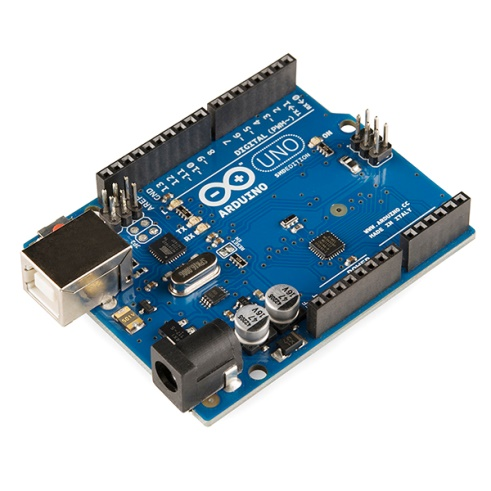
\includegraphics[width=0.3\textwidth]{figures/Introduccion/arduino.jpg}
			\caption{Placa Arduino}
			\label{fig.arduino}
	  		\end{center}
	\end{figure}
	
	\item Mbot: es un kit de robótica para que los niños se inicien en la robótica, programación y electrónica. Utiliza un  entorno de programación gráfica basada en Scratch 2.0
y es compatible con Arduino. Los niños pueden programar fácilmente el mBot sin escribir códigos y usar lenguajes de programación difíciles. Los usuarios también pueden usar la aplicación Makeblock para controlar sus robots.
	\begin{figure}[H]
  	  \begin{center}
    	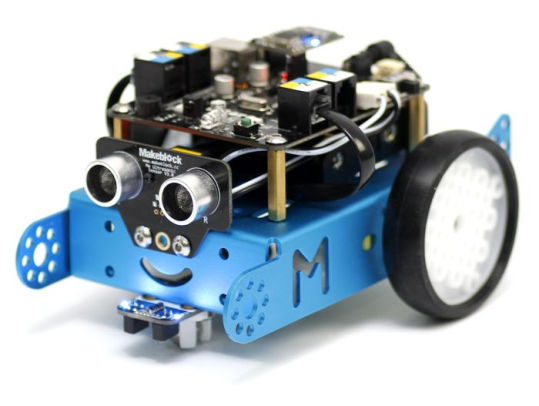
\includegraphics[width=0.3\textwidth]{figures/Introduccion/mbot.jpg}
			\caption{Robot mBot v1.1}
			\label{fig.mbot}
	  		\end{center}
	\end{figure}
\end{itemize}

\textbf{Plataformas software:} 
\begin{itemize}
	\item Scratch: Es un lenguaje de programación visual desarrollado por el MIT Media Lab. Desde 2013, Scratch 2 está disponible en línea y como aplicación de escritorio para Windows, OS X y Linux (requiere Adobe Air). Se empezó a usar Scratch como lenguaje introductorio por su relativa facilidad para desarrollar programas y  porque las habilidades adquiridas mediante Scratch se pueden aplicar a otros lenguajes básicos de programación como Python y Java. El uso de Scratch permite a las personas jóvenes a entender la lógica básica de la programación dirigida por eventos con múltiples objetos activos llamados sprites (llamados "objetos" en la versión en castellano de Scratch). Los sprites pueden pintarse como gráficos vectoriales o mapa de bits, desde la propia web de Scratch usando un simple editor que es parte del proyecto, o pueden también importarse desde fuentes externas incluyendo webcams.
	\item Lenguaje Arduino: Para decirle a la placa de Arduino qué hacer se utiliza el lenguaje de programación Arduino y su entorno de desarrollo. El software de código abierto Arduino (IDE) hace que sea fácil escribir código. Se ejecuta en Windows, Mac OS X y Linux. El entorno está escrito en Java y está basado en Processing. 
Este software se puede usar con cualquier placa Arduino.
\end{itemize}

Como entorno educativo, JdeRobot ha desarrollado JdeRobot-Kids. El objetivo principal del curso es enseñar conceptos básicos de tecnología a los alumnos e iniciarles en robótica y programación. También introduce de manera atractiva conceptos interesantes de mecánica, electrónica e informática. El carácter del curso es práctico y  ayuda a estructurar el pensamiento, a organizar las acciones en pasos para resolver un problema y a fomentar el espíritu analítico. Emplean dos plataformas concretas: ArduinoRobot y un Arduino estandard montado desde piezas y como lenguaje de programación Python y Scratch. 


\subsection{Robótica en universidades}

En la docencia universitaria se imparten clases de robótica en los Grados y los Postgrados, en concreto en escuelas de ingeniería. En España, se puede ver la robótica integrada en el ``Grado en Ingeniería Robótica'' de la Universidad de Alicante, y los Grados de ``Electrónica industrial y automática'' o en ``Ingeniería Electrónica, Robótica y Mecatrónica'' en diversas universidades. \\

En los estudios de Postgrado existen Másteres destacados como el ``Máster de Visión Artificial'' en diferentes universidades. \\

En el ámbito internacional se pueden destacar universidades especializadas en robótica como el MIT, Stanford, Georgia Institute of Technology, etc. \\

Cabe destacar el entorno de enseñanza robótica TheConstructSim \footnote{\url{http://www.theconstructsim.com/}} cuyo objetivo es enseñar a programar ROS.  Contiene una serie de tutoriales ROS en línea vinculados a simulaciones en línea, que brindan las herramientas y el conocimiento necesario para comprender y crear cualquier desarrollo de robótica basado en ROS. Usa robots reales simulados y solo se necesita un navegador web por lo que no requiere instalación.


\section{JdeRobot-Academy}
La Universidad Rey Juan Carlos cuenta con la plataforma de robótica JdeRobot, que posee un entorno académico conocido como JdeRobot-Academy. Este entorno educativo se ha empleado con éxito en diferentes asignaturas, como son ``Visión en Robótica'' del Máster de Visión Artificial, o ``Robótica'' del Grado de Ingeniería Telemática. Asimismo, la Universidad ofrece cursos de introducción a la robótica y a los drones, empleando dicha plataforma. \\

Está diseñado para que las prácticas, desarrolladas por los alumnos, se ejecuten en robots reales y también en simulados sin modificar el código fuente. El lenguaje de programación que se utiliza prácticas es Python debido a su sencillez y la potencia que ofrece. Para probar dichas prácticas en robots, se usa el simulador Gazebo. Este simulador permite aprender robótica aunque no se tengan los robots reales ya que dispone de una gran variedad de robots, como pueden ser drones, coches, aspiradoras o brazos mecánicos, entre otros, pudiendo abarcar distintos aspectos de la robótica. \\

Cada práctica consta de una aplicación académica, que resuelve tareas como la interfaz gráfica (GUI) o la conexión con sensores y actuadores concretos, y que queda oculta para el alumno. También contiene el código del estudiante, que simplemente rellena un sencillo fichero plantilla, llamado MyAlgorithm.py, con la lógica del robot, logrando así que se centre solamente en la creación y desarrollo de los algoritmos de percepción, planificación y control, habituales en los robots, necesarios para la resolución de la práctica. \\

\begin{figure}[H]
  \begin{center}
    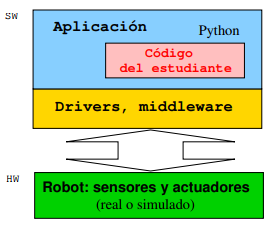
\includegraphics[width=0.5\textwidth]{figures/Introduccion/esquema.png}
		\caption{Diseño de una práctica robótica}
		\label{fig.esquema}
		\end{center}
\end{figure}

En la Figura~\ref{fig.esquema} se puede apreciar cómo está diseñada una práctica en el entorno de JdeRobot-Academy. En la capa inferior se encuentra el robot con sus actuadores (ruedas, motores...) y sensores (láseres, cámaras…) y puede ser tanto simulado como real.  En la capa intermedia se tienen los drivers y middlewares necesarios para la comunicación entre la aplicación y el robot. Y por último, en la capa superior, está la aplicación donde se analizan los datos captados por los sensores y se desarrolla el código del estudiante, tomando decisiones de actuación y planificación. \\

En la siguiente figura se puede ver la estructura que tiene cada una de las prácticas y como estan relacionados los distintos componentes.

\begin{figure}[H]
  \begin{center}
    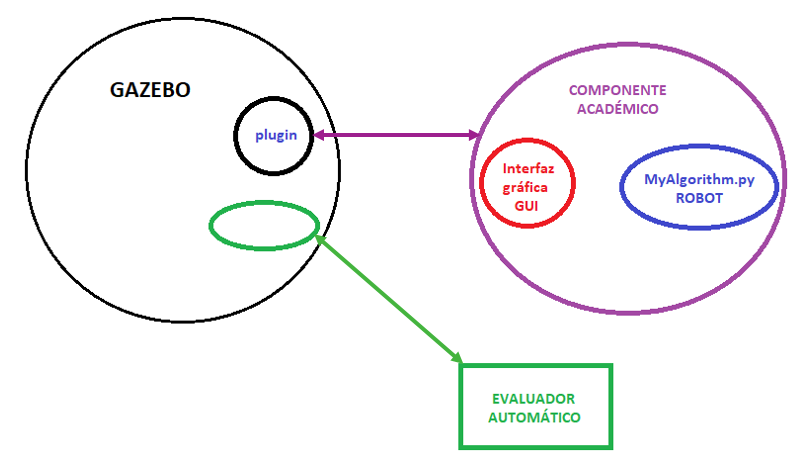
\includegraphics[width=0.9\textwidth]{figures/Introduccion/estructura.png}
		\caption{Estructura de una práctica robótica}
		\label{fig.estructura}
		\end{center}
\end{figure}


Los ámbitos principales en los que actualmente se han desarrollado prácticas son:
\begin{itemize}
	\item Visión: Aquí se pueden encontrar las prácticas ‘Color filter’, cuyo principal objetivo es el uso de filtros de color, y ‘Visual 3D reconstruction from a stereo pair of RGB cameras’ en la que se reconstruye una imagen en 3D a partir de dos cámaras de vídeo.
	\begin{figure}[H]
  	\begin{center}
    	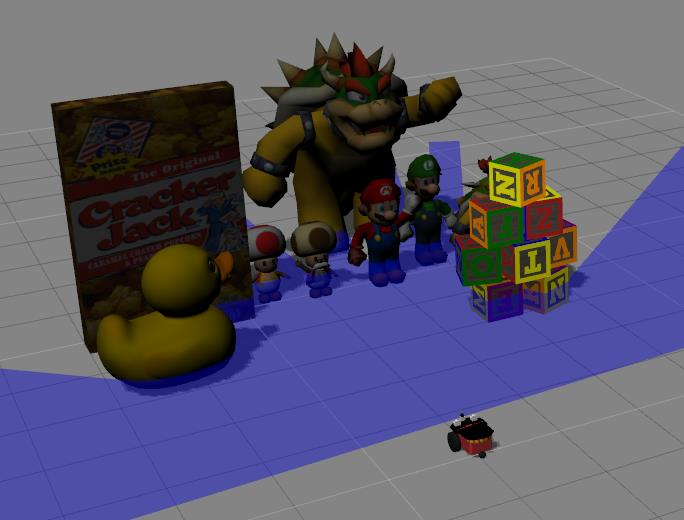
\includegraphics[width=0.4\textwidth]{figures/Introduccion/vision.jpg}
			\caption{Práctica ``Visual 3D reconstruction''}
			\label{fig.vision}
			\end{center}
	\end{figure}

	\item Coches autónomos: En este ámbito se han desarrollado las prácticas ``Visual follow-line behavior on a Formula 1'' en la cual los alumnos tienen que conseguir que un coche de Fórmula 1 logre seguir una línea roja pintada en un circuito de carreras; ``Local navigation of a Formula 1 with VFF'', su objetivo es que el alumno programe un algoritmo que consiga que un coche Fórmula 1 recorra un circuito evitando chocar con obstáculos (que son otros coches estacionados a lo largo del circuito); y ``Global navigation of a TeleTaxi with GPP'', en la cual el alumno debe programar un algoritmo para que un taxi consiga llegar a un punto del mundo en el que se encuentra clicando en una parte del mapa de dicho mundo.
	\begin{figure}[H]
  	\begin{center}
    	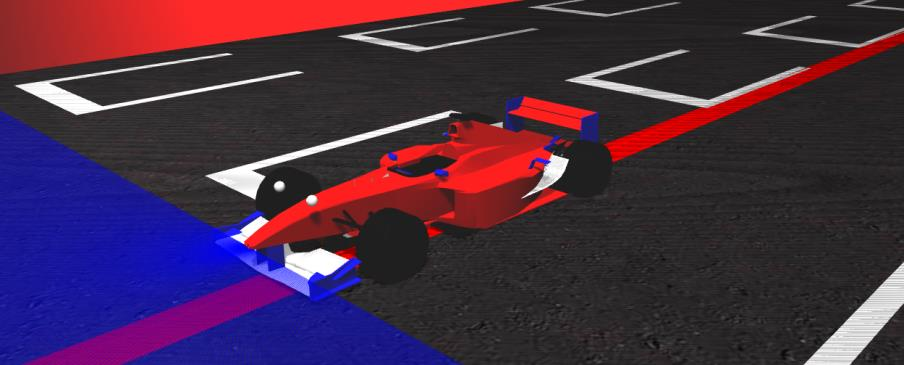
\includegraphics[width=0.4\textwidth]{figures/Introduccion/f1.jpg}
			\caption{Coche de Fórmula 1}
			\label{fig.f1}
			\end{center}
	\end{figure}

	\item Robots móviles: La práctica realizada es  ``Bump and go'', que consiste en programar la técnica ``choca-gira''  con un robot Kobuki.

	\item Drones: Es el ámbito que posee más prácticas desarrolladas. ``Drone position control navigation'' se basa en el uso de controladores PID; ``Follow the ground robot'', cuyo objetivo es conseguir que un dron siga a un robot Kobuki; ``Follow the road'', en la cual, un dron sigue una carretera; ``Drone cat and mouse'' que consiste en que un dron juega el papel de gato y tiene que atrapar al dron que tiene el papel de ratón; ``Landing on a moving car'', en esta práctica hay que lograr que un dron aterrice sobre un coche en movimiento; ``Escaping from a labyrinth using visual clue'', el objetivo es conseguir que un dron salga de un laberinto siguiendo las flechas ubicadas a lo largo de dicho laberinto; y ``People rescue after an earthquake'' que consiste en que un dron detecte personas y marque la posición en la que se encuentran.
\begin{figure}[H]
  	\begin{center}
    	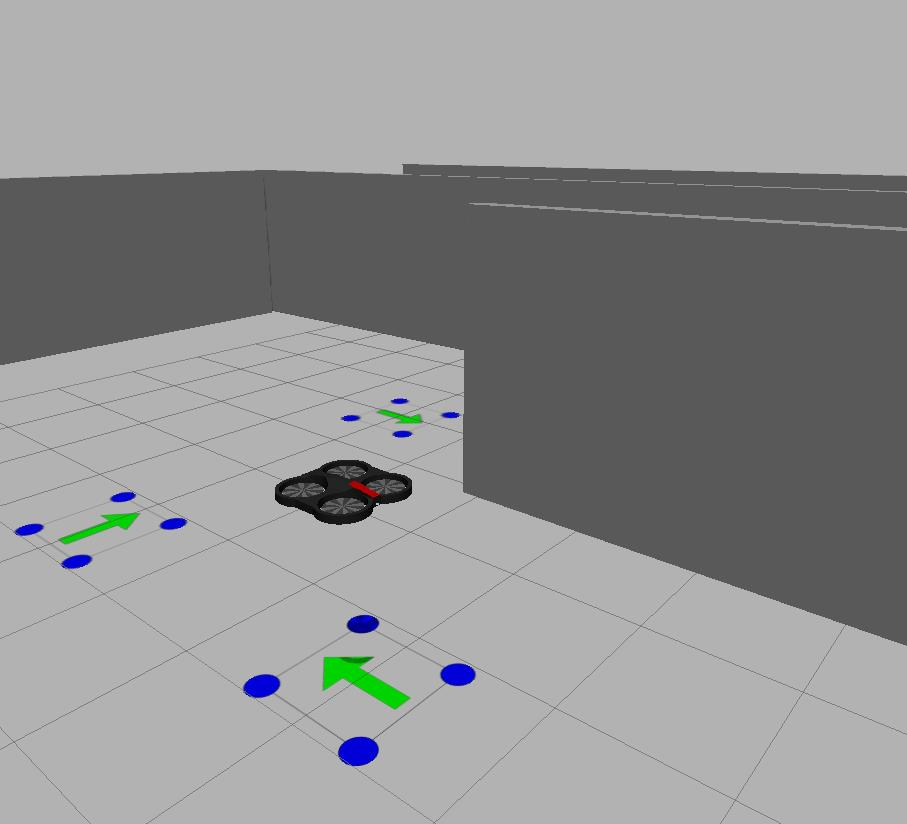
\includegraphics[width=0.4\textwidth]{figures/Introduccion/dron.jpg}
			\caption{Dron situado en un laberinto}
			\label{fig.dron}
			\end{center}
	\end{figure}
\end{itemize}
